\documentclass{standalone}
\usepackage{tikz}
\usetikzlibrary{patterns, positioning}


\begin{document}
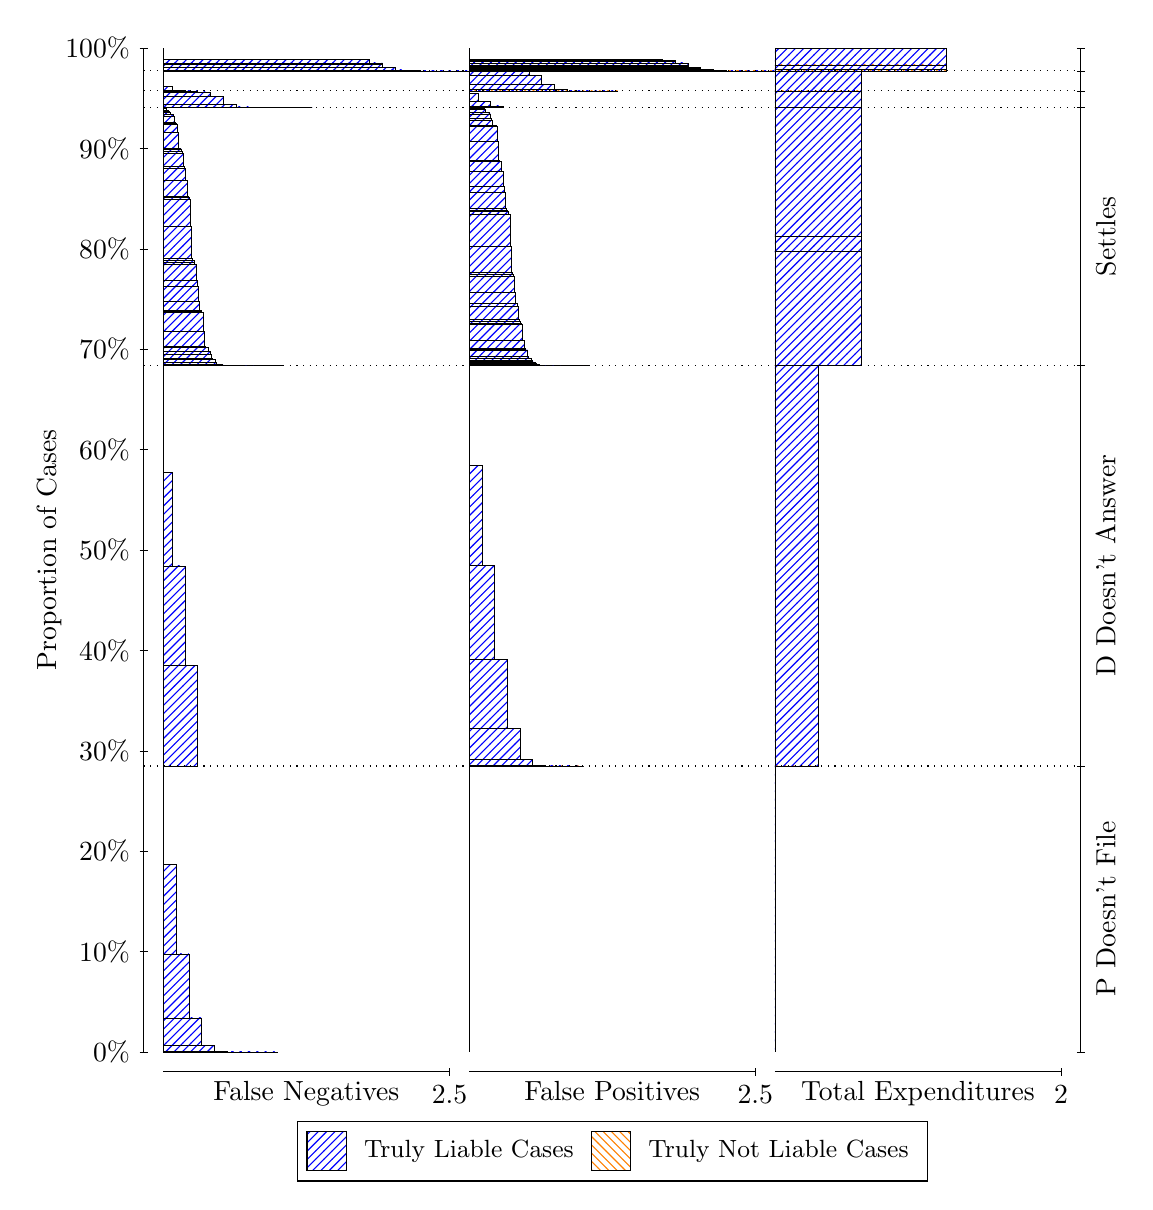
\begin{tikzpicture}
\draw[black, very thin] (1.5,1.75) -- (1.5,14.5);
\node[rotate=90, text=black, anchor=center] at (0.3, 8.125) {Proportion of Cases};
\draw[black, very thin] (1.45,1.75) -- (1.55,1.75);
\node[text=black, anchor=east] at (1.45, 1.75) {0\%};
\draw[black, very thin] (1.45,3.025) -- (1.55,3.025);
\node[text=black, anchor=east] at (1.45, 3.025) {10\%};
\draw[black, very thin] (1.45,4.3) -- (1.55,4.3);
\node[text=black, anchor=east] at (1.45, 4.3) {20\%};
\draw[black, very thin] (1.45,5.575) -- (1.55,5.575);
\node[text=black, anchor=east] at (1.45, 5.575) {30\%};
\draw[black, very thin] (1.45,6.85) -- (1.55,6.85);
\node[text=black, anchor=east] at (1.45, 6.85) {40\%};
\draw[black, very thin] (1.45,8.125) -- (1.55,8.125);
\node[text=black, anchor=east] at (1.45, 8.125) {50\%};
\draw[black, very thin] (1.45,9.4) -- (1.55,9.4);
\node[text=black, anchor=east] at (1.45, 9.4) {60\%};
\draw[black, very thin] (1.45,10.675) -- (1.55,10.675);
\node[text=black, anchor=east] at (1.45, 10.675) {70\%};
\draw[black, very thin] (1.45,11.95) -- (1.55,11.95);
\node[text=black, anchor=east] at (1.45, 11.95) {80\%};
\draw[black, very thin] (1.45,13.225) -- (1.55,13.225);
\node[text=black, anchor=east] at (1.45, 13.225) {90\%};
\draw[black, very thin] (1.45,14.5) -- (1.55,14.5);
\node[text=black, anchor=east] at (1.45, 14.5) {100\%};

\draw[black, very thin] (13.4,1.75) -- (13.4,14.5);
\draw[black, very thin] (13.35,1.75) -- (13.45,1.75);
\node[anchor=west] at (13.35, 1.75) {};
\draw[black, very thin] (13.35,5.382) -- (13.45,5.382);
\node[anchor=west] at (13.35, 5.382) {};
\draw[black, very thin] (13.35,10.471) -- (13.45,10.471);
\node[anchor=west] at (13.35, 10.471) {};
\draw[black, very thin] (13.35,13.75) -- (13.45,13.75);
\node[anchor=west] at (13.35, 13.75) {};
\draw[black, very thin] (13.35,13.956) -- (13.45,13.956);
\node[anchor=west] at (13.35, 13.956) {};
\draw[black, very thin] (13.35,14.211) -- (13.45,14.211);
\node[anchor=west] at (13.35, 14.211) {};
\draw[black, very thin] (13.35,14.5) -- (13.45,14.5);
\node[anchor=west] at (13.35, 14.5) {};

\draw[black, very thin, pattern color=blue, pattern=north east lines] (1.75,1.75) rectangle (3.2033,1.75);
\draw[black, very thin, pattern color=blue, pattern=north east lines] (1.75,1.75) rectangle (3.0419,1.75);
\draw[black, very thin, pattern color=blue, pattern=north east lines] (1.75,1.75) rectangle (2.8804,1.75);
\draw[black, very thin, pattern color=blue, pattern=north east lines] (1.75,1.75) rectangle (2.7189,1.7503);
\draw[black, very thin, pattern color=blue, pattern=north east lines] (1.75,1.7503) rectangle (2.5574,1.7572);
\draw[black, very thin, pattern color=blue, pattern=north east lines] (1.75,1.7572) rectangle (2.3959,1.8318);
\draw[black, very thin, pattern color=blue, pattern=north east lines] (1.75,1.8318) rectangle (2.2344,2.1829);
\draw[black, very thin, pattern color=blue, pattern=north east lines] (1.75,2.1829) rectangle (2.073,2.995);
\draw[black, very thin, pattern color=blue, pattern=north east lines] (1.75,2.995) rectangle (1.9115,4.1337);
\draw[black, very thin, pattern color=orange, pattern=north west lines] (1.75,4.1337) rectangle (1.75,4.1337);
\draw[black, very thin, pattern color=blue, pattern=north east lines] (1.75,4.1337) rectangle (1.75,5.382);
\draw[black, very thin, pattern color=blue, pattern=north east lines] (1.75,5.382) rectangle (2.186,6.6566);
\draw[black, very thin, pattern color=blue, pattern=north east lines] (1.75,6.6566) rectangle (2.0245,7.9231);
\draw[black, very thin, pattern color=blue, pattern=north east lines] (1.75,7.9231) rectangle (1.863,9.1124);
\draw[black, very thin, pattern color=orange, pattern=north west lines] (1.75,9.1124) rectangle (1.75,9.1124);
\draw[black, very thin, pattern color=blue, pattern=north east lines] (1.75,9.1124) rectangle (1.75,10.471);
\draw[black, very thin, pattern color=blue, pattern=north east lines] (1.75,10.471) rectangle (3.276,10.471);
\draw[black, very thin, pattern color=blue, pattern=north east lines] (1.75,10.471) rectangle (3.2033,10.471);
\draw[black, very thin, pattern color=blue, pattern=north east lines] (1.75,10.471) rectangle (3.1307,10.471);
\draw[black, very thin, pattern color=blue, pattern=north east lines] (1.75,10.471) rectangle (3.1145,10.471);
\draw[black, very thin, pattern color=blue, pattern=north east lines] (1.75,10.471) rectangle (3.058,10.471);
\draw[black, very thin, pattern color=blue, pattern=north east lines] (1.75,10.471) rectangle (3.0419,10.471);
\draw[black, very thin, pattern color=blue, pattern=north east lines] (1.75,10.471) rectangle (2.9853,10.471);
\draw[black, very thin, pattern color=blue, pattern=north east lines] (1.75,10.471) rectangle (2.9692,10.471);
\draw[black, very thin, pattern color=blue, pattern=north east lines] (1.75,10.471) rectangle (2.953,10.471);
\draw[black, very thin, pattern color=blue, pattern=north east lines] (1.75,10.471) rectangle (2.9127,10.471);
\draw[black, very thin, pattern color=blue, pattern=north east lines] (1.75,10.471) rectangle (2.8965,10.471);
\draw[black, very thin, pattern color=blue, pattern=north east lines] (1.75,10.471) rectangle (2.8804,10.471);
\draw[black, very thin, pattern color=blue, pattern=north east lines] (1.75,10.471) rectangle (2.84,10.471);
\draw[black, very thin, pattern color=blue, pattern=north east lines] (1.75,10.471) rectangle (2.8239,10.471);
\draw[black, very thin, pattern color=blue, pattern=north east lines] (1.75,10.471) rectangle (2.8077,10.471);
\draw[black, very thin, pattern color=blue, pattern=north east lines] (1.75,10.471) rectangle (2.7916,10.471);
\draw[black, very thin, pattern color=blue, pattern=north east lines] (1.75,10.471) rectangle (2.7673,10.471);
\draw[black, very thin, pattern color=blue, pattern=north east lines] (1.75,10.471) rectangle (2.7512,10.471);
\draw[black, very thin, pattern color=blue, pattern=north east lines] (1.75,10.471) rectangle (2.735,10.471);
\draw[black, very thin, pattern color=blue, pattern=north east lines] (1.75,10.471) rectangle (2.7189,10.471);
\draw[black, very thin, pattern color=blue, pattern=north east lines] (1.75,10.471) rectangle (2.6947,10.471);
\draw[black, very thin, pattern color=blue, pattern=north east lines] (1.75,10.471) rectangle (2.6785,10.471);
\draw[black, very thin, pattern color=blue, pattern=north east lines] (1.75,10.471) rectangle (2.6624,10.471);
\draw[black, very thin, pattern color=blue, pattern=north east lines] (1.75,10.471) rectangle (2.6462,10.471);
\draw[black, very thin, pattern color=blue, pattern=north east lines] (1.75,10.471) rectangle (2.6301,10.471);
\draw[black, very thin, pattern color=blue, pattern=north east lines] (1.75,10.471) rectangle (2.622,10.471);
\draw[black, very thin, pattern color=blue, pattern=north east lines] (1.75,10.471) rectangle (2.6059,10.471);
\draw[black, very thin, pattern color=blue, pattern=north east lines] (1.75,10.471) rectangle (2.5897,10.472);
\draw[black, very thin, pattern color=blue, pattern=north east lines] (1.75,10.472) rectangle (2.5736,10.473);
\draw[black, very thin, pattern color=blue, pattern=north east lines] (1.75,10.473) rectangle (2.5574,10.473);
\draw[black, very thin, pattern color=blue, pattern=north east lines] (1.75,10.473) rectangle (2.5493,10.473);
\draw[black, very thin, pattern color=blue, pattern=north east lines] (1.75,10.473) rectangle (2.5332,10.473);
\draw[black, very thin, pattern color=blue, pattern=north east lines] (1.75,10.473) rectangle (2.517,10.476);
\draw[black, very thin, pattern color=blue, pattern=north east lines] (1.75,10.476) rectangle (2.5009,10.479);
\draw[black, very thin, pattern color=blue, pattern=north east lines] (1.75,10.479) rectangle (2.4847,10.482);
\draw[black, very thin, pattern color=blue, pattern=north east lines] (1.75,10.482) rectangle (2.4686,10.482);
\draw[black, very thin, pattern color=blue, pattern=north east lines] (1.75,10.482) rectangle (2.4605,10.482);
\draw[black, very thin, pattern color=blue, pattern=north east lines] (1.75,10.482) rectangle (2.4444,10.483);
\draw[black, very thin, pattern color=blue, pattern=north east lines] (1.75,10.483) rectangle (2.4282,10.503);
\draw[black, very thin, pattern color=blue, pattern=north east lines] (1.75,10.503) rectangle (2.4121,10.541);
\draw[black, very thin, pattern color=blue, pattern=north east lines] (1.75,10.541) rectangle (2.3959,10.541);
\draw[black, very thin, pattern color=blue, pattern=north east lines] (1.75,10.541) rectangle (2.3879,10.542);
\draw[black, very thin, pattern color=blue, pattern=north east lines] (1.75,10.542) rectangle (2.3717,10.556);
\draw[black, very thin, pattern color=blue, pattern=north east lines] (1.75,10.556) rectangle (2.3556,10.612);
\draw[black, very thin, pattern color=blue, pattern=north east lines] (1.75,10.612) rectangle (2.3394,10.644);
\draw[black, very thin, pattern color=blue, pattern=north east lines] (1.75,10.644) rectangle (2.3233,10.696);
\draw[black, very thin, pattern color=blue, pattern=north east lines] (1.75,10.696) rectangle (2.3071,10.699);
\draw[black, very thin, pattern color=blue, pattern=north east lines] (1.75,10.699) rectangle (2.299,10.702);
\draw[black, very thin, pattern color=blue, pattern=north east lines] (1.75,10.702) rectangle (2.2829,10.712);
\draw[black, very thin, pattern color=blue, pattern=north east lines] (1.75,10.712) rectangle (2.2667,10.909);
\draw[black, very thin, pattern color=blue, pattern=north east lines] (1.75,10.909) rectangle (2.2506,11.147);
\draw[black, very thin, pattern color=blue, pattern=north east lines] (1.75,11.147) rectangle (2.2344,11.158);
\draw[black, very thin, pattern color=blue, pattern=north east lines] (1.75,11.158) rectangle (2.2264,11.164);
\draw[black, very thin, pattern color=blue, pattern=north east lines] (1.75,11.164) rectangle (2.2102,11.28);
\draw[black, very thin, pattern color=blue, pattern=north east lines] (1.75,11.28) rectangle (2.1941,11.48);
\draw[black, very thin, pattern color=blue, pattern=north east lines] (1.75,11.48) rectangle (2.1779,11.549);
\draw[black, very thin, pattern color=blue, pattern=north east lines] (1.75,11.549) rectangle (2.1618,11.759);
\draw[black, very thin, pattern color=blue, pattern=north east lines] (1.75,11.759) rectangle (2.1456,11.777);
\draw[black, very thin, pattern color=blue, pattern=north east lines] (1.75,11.777) rectangle (2.1376,11.8);
\draw[black, very thin, pattern color=blue, pattern=north east lines] (1.75,11.8) rectangle (2.1214,11.826);
\draw[black, very thin, pattern color=blue, pattern=north east lines] (1.75,11.826) rectangle (2.1053,12.239);
\draw[black, very thin, pattern color=blue, pattern=north east lines] (1.75,12.239) rectangle (2.0891,12.573);
\draw[black, very thin, pattern color=blue, pattern=north east lines] (1.75,12.573) rectangle (2.073,12.599);
\draw[black, very thin, pattern color=blue, pattern=north east lines] (1.75,12.599) rectangle (2.0649,12.619);
\draw[black, very thin, pattern color=blue, pattern=north east lines] (1.75,12.619) rectangle (2.0487,12.819);
\draw[black, very thin, pattern color=blue, pattern=north east lines] (1.75,12.819) rectangle (2.0326,12.967);
\draw[black, very thin, pattern color=blue, pattern=north east lines] (1.75,12.967) rectangle (2.0164,13);
\draw[black, very thin, pattern color=blue, pattern=north east lines] (1.75,13) rectangle (2.0003,13.166);
\draw[black, very thin, pattern color=blue, pattern=north east lines] (1.75,13.166) rectangle (1.9841,13.19);
\draw[black, very thin, pattern color=blue, pattern=north east lines] (1.75,13.19) rectangle (1.9761,13.22);
\draw[black, very thin, pattern color=blue, pattern=north east lines] (1.75,13.22) rectangle (1.9599,13.231);
\draw[black, very thin, pattern color=blue, pattern=north east lines] (1.75,13.231) rectangle (1.9438,13.434);
\draw[black, very thin, pattern color=blue, pattern=north east lines] (1.75,13.434) rectangle (1.9276,13.531);
\draw[black, very thin, pattern color=blue, pattern=north east lines] (1.75,13.531) rectangle (1.9115,13.543);
\draw[black, very thin, pattern color=blue, pattern=north east lines] (1.75,13.543) rectangle (1.9034,13.554);
\draw[black, very thin, pattern color=blue, pattern=north east lines] (1.75,13.554) rectangle (1.8873,13.636);
\draw[black, very thin, pattern color=blue, pattern=north east lines] (1.75,13.636) rectangle (1.8711,13.659);
\draw[black, very thin, pattern color=blue, pattern=north east lines] (1.75,13.659) rectangle (1.855,13.664);
\draw[black, very thin, pattern color=blue, pattern=north east lines] (1.75,13.664) rectangle (1.8388,13.69);
\draw[black, very thin, pattern color=blue, pattern=north east lines] (1.75,13.69) rectangle (1.8227,13.7);
\draw[black, very thin, pattern color=blue, pattern=north east lines] (1.75,13.7) rectangle (1.8146,13.708);
\draw[black, very thin, pattern color=blue, pattern=north east lines] (1.75,13.708) rectangle (1.7984,13.708);
\draw[black, very thin, pattern color=blue, pattern=north east lines] (1.75,13.708) rectangle (1.7823,13.73);
\draw[black, very thin, pattern color=blue, pattern=north east lines] (1.75,13.73) rectangle (1.7661,13.736);
\draw[black, very thin, pattern color=orange, pattern=north west lines] (1.75,13.736) rectangle (1.75,13.736);
\draw[black, very thin, pattern color=blue, pattern=north east lines] (1.75,13.736) rectangle (1.75,13.75);
\draw[black, very thin, pattern color=blue, pattern=north east lines] (1.75,13.75) rectangle (3.6393,13.75);
\draw[black, very thin, pattern color=blue, pattern=north east lines] (1.75,13.75) rectangle (3.4779,13.75);
\draw[black, very thin, pattern color=blue, pattern=north east lines] (1.75,13.75) rectangle (3.3164,13.75);
\draw[black, very thin, pattern color=blue, pattern=north east lines] (1.75,13.75) rectangle (3.1549,13.75);
\draw[black, very thin, pattern color=blue, pattern=north east lines] (1.75,13.75) rectangle (2.9934,13.75);
\draw[black, very thin, pattern color=blue, pattern=north east lines] (1.75,13.75) rectangle (2.8319,13.752);
\draw[black, very thin, pattern color=blue, pattern=north east lines] (1.75,13.752) rectangle (2.6704,13.785);
\draw[black, very thin, pattern color=blue, pattern=north east lines] (1.75,13.785) rectangle (2.509,13.881);
\draw[black, very thin, pattern color=blue, pattern=north east lines] (1.75,13.881) rectangle (2.3475,13.942);
\draw[black, very thin, pattern color=blue, pattern=north east lines] (1.75,13.942) rectangle (2.186,13.956);
\draw[black, very thin, pattern color=orange, pattern=north west lines] (1.75,13.956) rectangle (1.75,13.956);
\draw[black, very thin, pattern color=blue, pattern=north east lines] (1.75,13.956) rectangle (2.186,13.956);
\draw[black, very thin, pattern color=blue, pattern=north east lines] (1.75,13.956) rectangle (2.0245,13.963);
\draw[black, very thin, pattern color=blue, pattern=north east lines] (1.75,13.963) rectangle (1.863,14.015);
\draw[black, very thin, pattern color=orange, pattern=north west lines] (1.75,14.015) rectangle (1.75,14.015);
\draw[black, very thin, pattern color=blue, pattern=north east lines] (1.75,14.015) rectangle (1.75,14.211);
\draw[black, very thin, pattern color=blue, pattern=north east lines] (1.75,14.211) rectangle (5.8193,14.211);
\draw[black, very thin, pattern color=blue, pattern=north east lines] (1.75,14.211) rectangle (5.6579,14.211);
\draw[black, very thin, pattern color=blue, pattern=north east lines] (1.75,14.211) rectangle (5.4964,14.211);
\draw[black, very thin, pattern color=blue, pattern=north east lines] (1.75,14.211) rectangle (5.3349,14.211);
\draw[black, very thin, pattern color=blue, pattern=north east lines] (1.75,14.211) rectangle (5.3349,14.211);
\draw[black, very thin, pattern color=blue, pattern=north east lines] (1.75,14.211) rectangle (5.1734,14.211);
\draw[black, very thin, pattern color=blue, pattern=north east lines] (1.75,14.211) rectangle (5.0119,14.212);
\draw[black, very thin, pattern color=blue, pattern=north east lines] (1.75,14.212) rectangle (5.0119,14.212);
\draw[black, very thin, pattern color=blue, pattern=north east lines] (1.75,14.212) rectangle (4.8504,14.216);
\draw[black, very thin, pattern color=blue, pattern=north east lines] (1.75,14.216) rectangle (4.8504,14.222);
\draw[black, very thin, pattern color=blue, pattern=north east lines] (1.75,14.222) rectangle (4.689,14.254);
\draw[black, very thin, pattern color=blue, pattern=north east lines] (1.75,14.254) rectangle (4.5275,14.298);
\draw[black, very thin, pattern color=blue, pattern=north east lines] (1.75,14.298) rectangle (4.5275,14.31);
\draw[black, very thin, pattern color=blue, pattern=north east lines] (1.75,14.31) rectangle (4.366,14.351);
\draw[black, very thin, pattern color=blue, pattern=north east lines] (1.75,14.351) rectangle (4.2045,14.351);
\draw[black, very thin, pattern color=blue, pattern=north east lines] (1.75,14.351) rectangle (4.2045,14.358);
\draw[black, very thin, pattern color=blue, pattern=north east lines] (1.75,14.358) rectangle (4.043,14.358);
\draw[black, very thin, pattern color=blue, pattern=north east lines] (1.75,14.358) rectangle (4.043,14.358);
\draw[black, very thin, pattern color=blue, pattern=north east lines] (1.75,14.358) rectangle (3.8816,14.358);
\draw[black, very thin, pattern color=blue, pattern=north east lines] (1.75,14.358) rectangle (3.8816,14.358);
\draw[black, very thin, pattern color=blue, pattern=north east lines] (1.75,14.358) rectangle (3.7201,14.358);
\draw[black, very thin, pattern color=blue, pattern=north east lines] (1.75,14.358) rectangle (3.7201,14.358);
\draw[black, very thin, pattern color=blue, pattern=north east lines] (1.75,14.358) rectangle (3.5586,14.358);
\draw[black, very thin, pattern color=blue, pattern=north east lines] (1.75,14.358) rectangle (3.5586,14.358);
\draw[black, very thin, pattern color=blue, pattern=north east lines] (1.75,14.358) rectangle (3.3971,14.358);
\draw[black, very thin, pattern color=blue, pattern=north east lines] (1.75,14.358) rectangle (2.0084,14.358);
\draw[black, very thin, pattern color=blue, pattern=north east lines] (1.75,14.358) rectangle (1.8469,14.358);
\draw[black, very thin, pattern color=orange, pattern=north west lines] (1.75,14.358) rectangle (1.75,14.358);
\draw[black, very thin, pattern color=blue, pattern=north east lines] (1.75,14.358) rectangle (1.75,14.5);
\draw[black, very thin, pattern color=orange, pattern=north west lines] (5.6333,1.75) rectangle (5.6333,1.75);
\draw[black, very thin, pattern color=blue, pattern=north east lines] (5.6333,1.75) rectangle (5.6333,5.382);
\draw[black, very thin, pattern color=orange, pattern=north west lines] (5.6333,5.382) rectangle (7.0867,5.382);
\draw[black, very thin, pattern color=blue, pattern=north east lines] (5.6333,5.382) rectangle (7.0867,5.382);
\draw[black, very thin, pattern color=blue, pattern=north east lines] (5.6333,5.382) rectangle (6.9252,5.382);
\draw[black, very thin, pattern color=blue, pattern=north east lines] (5.6333,5.382) rectangle (6.7637,5.3821);
\draw[black, very thin, pattern color=blue, pattern=north east lines] (5.6333,5.3821) rectangle (6.6022,5.3878);
\draw[black, very thin, pattern color=blue, pattern=north east lines] (5.6333,5.3878) rectangle (6.4407,5.468);
\draw[black, very thin, pattern color=blue, pattern=north east lines] (5.6333,5.468) rectangle (6.2793,5.8593);
\draw[black, very thin, pattern color=blue, pattern=north east lines] (5.6333,5.8593) rectangle (6.1178,6.7406);
\draw[black, very thin, pattern color=blue, pattern=north east lines] (5.6333,6.7406) rectangle (5.9563,7.9299);
\draw[black, very thin, pattern color=blue, pattern=north east lines] (5.6333,7.9299) rectangle (5.7948,9.1965);
\draw[black, very thin, pattern color=blue, pattern=north east lines] (5.6333,9.1965) rectangle (5.6333,10.471);
\draw[black, very thin, pattern color=orange, pattern=north west lines] (5.6333,10.471) rectangle (7.1593,10.471);
\draw[black, very thin, pattern color=blue, pattern=north east lines] (5.6333,10.471) rectangle (7.1593,10.471);
\draw[black, very thin, pattern color=orange, pattern=north west lines] (5.6333,10.471) rectangle (7.0867,10.471);
\draw[black, very thin, pattern color=blue, pattern=north east lines] (5.6333,10.471) rectangle (7.0867,10.471);
\draw[black, very thin, pattern color=orange, pattern=north west lines] (5.6333,10.471) rectangle (7.014,10.471);
\draw[black, very thin, pattern color=blue, pattern=north east lines] (5.6333,10.471) rectangle (7.014,10.471);
\draw[black, very thin, pattern color=blue, pattern=north east lines] (5.6333,10.471) rectangle (6.9979,10.471);
\draw[black, very thin, pattern color=orange, pattern=north west lines] (5.6333,10.471) rectangle (6.9413,10.471);
\draw[black, very thin, pattern color=blue, pattern=north east lines] (5.6333,10.471) rectangle (6.9413,10.471);
\draw[black, very thin, pattern color=blue, pattern=north east lines] (5.6333,10.471) rectangle (6.9252,10.471);
\draw[black, very thin, pattern color=orange, pattern=north west lines] (5.6333,10.471) rectangle (6.8687,10.471);
\draw[black, very thin, pattern color=blue, pattern=north east lines] (5.6333,10.471) rectangle (6.8687,10.471);
\draw[black, very thin, pattern color=blue, pattern=north east lines] (5.6333,10.471) rectangle (6.8525,10.471);
\draw[black, very thin, pattern color=blue, pattern=north east lines] (5.6333,10.471) rectangle (6.8364,10.471);
\draw[black, very thin, pattern color=orange, pattern=north west lines] (5.6333,10.471) rectangle (6.796,10.471);
\draw[black, very thin, pattern color=blue, pattern=north east lines] (5.6333,10.471) rectangle (6.796,10.471);
\draw[black, very thin, pattern color=blue, pattern=north east lines] (5.6333,10.471) rectangle (6.7799,10.471);
\draw[black, very thin, pattern color=blue, pattern=north east lines] (5.6333,10.471) rectangle (6.7637,10.471);
\draw[black, very thin, pattern color=orange, pattern=north west lines] (5.6333,10.471) rectangle (6.7233,10.471);
\draw[black, very thin, pattern color=blue, pattern=north east lines] (5.6333,10.471) rectangle (6.7233,10.471);
\draw[black, very thin, pattern color=blue, pattern=north east lines] (5.6333,10.471) rectangle (6.7072,10.471);
\draw[black, very thin, pattern color=blue, pattern=north east lines] (5.6333,10.471) rectangle (6.691,10.471);
\draw[black, very thin, pattern color=blue, pattern=north east lines] (5.6333,10.471) rectangle (6.6749,10.471);
\draw[black, very thin, pattern color=orange, pattern=north west lines] (5.6333,10.471) rectangle (6.6507,10.471);
\draw[black, very thin, pattern color=blue, pattern=north east lines] (5.6333,10.471) rectangle (6.6507,10.471);
\draw[black, very thin, pattern color=blue, pattern=north east lines] (5.6333,10.471) rectangle (6.6345,10.472);
\draw[black, very thin, pattern color=blue, pattern=north east lines] (5.6333,10.472) rectangle (6.6184,10.472);
\draw[black, very thin, pattern color=blue, pattern=north east lines] (5.6333,10.472) rectangle (6.6022,10.472);
\draw[black, very thin, pattern color=orange, pattern=north west lines] (5.6333,10.472) rectangle (6.578,10.472);
\draw[black, very thin, pattern color=blue, pattern=north east lines] (5.6333,10.472) rectangle (6.578,10.473);
\draw[black, very thin, pattern color=blue, pattern=north east lines] (5.6333,10.473) rectangle (6.5619,10.474);
\draw[black, very thin, pattern color=blue, pattern=north east lines] (5.6333,10.474) rectangle (6.5457,10.474);
\draw[black, very thin, pattern color=blue, pattern=north east lines] (5.6333,10.474) rectangle (6.5296,10.482);
\draw[black, very thin, pattern color=blue, pattern=north east lines] (5.6333,10.482) rectangle (6.5134,10.483);
\draw[black, very thin, pattern color=orange, pattern=north west lines] (5.6333,10.483) rectangle (6.5053,10.483);
\draw[black, very thin, pattern color=blue, pattern=north east lines] (5.6333,10.483) rectangle (6.5053,10.485);
\draw[black, very thin, pattern color=blue, pattern=north east lines] (5.6333,10.485) rectangle (6.4892,10.491);
\draw[black, very thin, pattern color=blue, pattern=north east lines] (5.6333,10.491) rectangle (6.473,10.513);
\draw[black, very thin, pattern color=blue, pattern=north east lines] (5.6333,10.513) rectangle (6.4569,10.513);
\draw[black, very thin, pattern color=blue, pattern=north east lines] (5.6333,10.513) rectangle (6.4407,10.521);
\draw[black, very thin, pattern color=orange, pattern=north west lines] (5.6333,10.521) rectangle (6.4327,10.521);
\draw[black, very thin, pattern color=blue, pattern=north east lines] (5.6333,10.521) rectangle (6.4327,10.531);
\draw[black, very thin, pattern color=blue, pattern=north east lines] (5.6333,10.531) rectangle (6.4165,10.557);
\draw[black, very thin, pattern color=blue, pattern=north east lines] (5.6333,10.557) rectangle (6.4004,10.562);
\draw[black, very thin, pattern color=blue, pattern=north east lines] (5.6333,10.562) rectangle (6.3842,10.585);
\draw[black, very thin, pattern color=blue, pattern=north east lines] (5.6333,10.585) rectangle (6.3681,10.667);
\draw[black, very thin, pattern color=blue, pattern=north east lines] (5.6333,10.667) rectangle (6.3519,10.678);
\draw[black, very thin, pattern color=blue, pattern=north east lines] (5.6333,10.678) rectangle (6.3439,10.69);
\draw[black, very thin, pattern color=blue, pattern=north east lines] (5.6333,10.69) rectangle (6.3277,10.787);
\draw[black, very thin, pattern color=blue, pattern=north east lines] (5.6333,10.787) rectangle (6.3116,10.99);
\draw[black, very thin, pattern color=blue, pattern=north east lines] (5.6333,10.99) rectangle (6.2954,11.001);
\draw[black, very thin, pattern color=blue, pattern=north east lines] (5.6333,11.001) rectangle (6.2793,11.031);
\draw[black, very thin, pattern color=blue, pattern=north east lines] (5.6333,11.031) rectangle (6.2712,11.055);
\draw[black, very thin, pattern color=blue, pattern=north east lines] (5.6333,11.055) rectangle (6.255,11.221);
\draw[black, very thin, pattern color=blue, pattern=north east lines] (5.6333,11.221) rectangle (6.2389,11.254);
\draw[black, very thin, pattern color=blue, pattern=north east lines] (5.6333,11.254) rectangle (6.2227,11.402);
\draw[black, very thin, pattern color=blue, pattern=north east lines] (5.6333,11.402) rectangle (6.2066,11.602);
\draw[black, very thin, pattern color=blue, pattern=north east lines] (5.6333,11.602) rectangle (6.1904,11.622);
\draw[black, very thin, pattern color=blue, pattern=north east lines] (5.6333,11.622) rectangle (6.1824,11.648);
\draw[black, very thin, pattern color=blue, pattern=north east lines] (5.6333,11.648) rectangle (6.1662,11.982);
\draw[black, very thin, pattern color=blue, pattern=north east lines] (5.6333,11.982) rectangle (6.1501,12.395);
\draw[black, very thin, pattern color=blue, pattern=north east lines] (5.6333,12.395) rectangle (6.1339,12.421);
\draw[black, very thin, pattern color=blue, pattern=north east lines] (5.6333,12.421) rectangle (6.1178,12.444);
\draw[black, very thin, pattern color=blue, pattern=north east lines] (5.6333,12.444) rectangle (6.1097,12.462);
\draw[black, very thin, pattern color=blue, pattern=north east lines] (5.6333,12.462) rectangle (6.0936,12.672);
\draw[black, very thin, pattern color=blue, pattern=north east lines] (5.6333,12.672) rectangle (6.0774,12.741);
\draw[black, very thin, pattern color=blue, pattern=north east lines] (5.6333,12.741) rectangle (6.0613,12.941);
\draw[black, very thin, pattern color=blue, pattern=north east lines] (5.6333,12.941) rectangle (6.0451,13.057);
\draw[black, very thin, pattern color=blue, pattern=north east lines] (5.6333,13.057) rectangle (6.029,13.063);
\draw[black, very thin, pattern color=blue, pattern=north east lines] (5.6333,13.063) rectangle (6.0209,13.074);
\draw[black, very thin, pattern color=blue, pattern=north east lines] (5.6333,13.074) rectangle (6.0047,13.312);
\draw[black, very thin, pattern color=blue, pattern=north east lines] (5.6333,13.312) rectangle (5.9886,13.509);
\draw[black, very thin, pattern color=blue, pattern=north east lines] (5.6333,13.509) rectangle (5.9724,13.519);
\draw[black, very thin, pattern color=blue, pattern=north east lines] (5.6333,13.519) rectangle (5.9563,13.522);
\draw[black, very thin, pattern color=blue, pattern=north east lines] (5.6333,13.522) rectangle (5.9482,13.525);
\draw[black, very thin, pattern color=blue, pattern=north east lines] (5.6333,13.525) rectangle (5.9321,13.577);
\draw[black, very thin, pattern color=blue, pattern=north east lines] (5.6333,13.577) rectangle (5.9159,13.609);
\draw[black, very thin, pattern color=blue, pattern=north east lines] (5.6333,13.609) rectangle (5.8998,13.665);
\draw[black, very thin, pattern color=blue, pattern=north east lines] (5.6333,13.665) rectangle (5.8836,13.679);
\draw[black, very thin, pattern color=blue, pattern=north east lines] (5.6333,13.679) rectangle (5.8675,13.68);
\draw[black, very thin, pattern color=blue, pattern=north east lines] (5.6333,13.68) rectangle (5.8594,13.68);
\draw[black, very thin, pattern color=blue, pattern=north east lines] (5.6333,13.68) rectangle (5.8433,13.718);
\draw[black, very thin, pattern color=blue, pattern=north east lines] (5.6333,13.718) rectangle (5.8271,13.738);
\draw[black, very thin, pattern color=blue, pattern=north east lines] (5.6333,13.738) rectangle (5.811,13.739);
\draw[black, very thin, pattern color=blue, pattern=north east lines] (5.6333,13.739) rectangle (5.7948,13.739);
\draw[black, very thin, pattern color=blue, pattern=north east lines] (5.6333,13.739) rectangle (5.7867,13.739);
\draw[black, very thin, pattern color=blue, pattern=north east lines] (5.6333,13.739) rectangle (5.7706,13.742);
\draw[black, very thin, pattern color=blue, pattern=north east lines] (5.6333,13.742) rectangle (5.7544,13.745);
\draw[black, very thin, pattern color=blue, pattern=north east lines] (5.6333,13.745) rectangle (5.7383,13.748);
\draw[black, very thin, pattern color=blue, pattern=north east lines] (5.6333,13.748) rectangle (5.7221,13.748);
\draw[black, very thin, pattern color=blue, pattern=north east lines] (5.6333,13.748) rectangle (5.706,13.748);
\draw[black, very thin, pattern color=blue, pattern=north east lines] (5.6333,13.748) rectangle (5.6979,13.748);
\draw[black, very thin, pattern color=blue, pattern=north east lines] (5.6333,13.748) rectangle (5.6818,13.749);
\draw[black, very thin, pattern color=blue, pattern=north east lines] (5.6333,13.749) rectangle (5.6656,13.75);
\draw[black, very thin, pattern color=blue, pattern=north east lines] (5.6333,13.75) rectangle (5.6495,13.75);
\draw[black, very thin, pattern color=blue, pattern=north east lines] (5.6333,13.75) rectangle (5.6333,13.75);
\draw[black, very thin, pattern color=orange, pattern=north west lines] (5.6333,13.75) rectangle (6.0693,13.75);
\draw[black, very thin, pattern color=blue, pattern=north east lines] (5.6333,13.75) rectangle (6.0693,13.764);
\draw[black, very thin, pattern color=blue, pattern=north east lines] (5.6333,13.764) rectangle (5.9079,13.825);
\draw[black, very thin, pattern color=blue, pattern=north east lines] (5.6333,13.825) rectangle (5.7464,13.921);
\draw[black, very thin, pattern color=blue, pattern=north east lines] (5.6333,13.921) rectangle (5.6333,13.956);
\draw[black, very thin, pattern color=orange, pattern=north west lines] (5.6333,13.956) rectangle (7.5227,13.956);
\draw[black, very thin, pattern color=blue, pattern=north east lines] (5.6333,13.956) rectangle (7.5227,13.956);
\draw[black, very thin, pattern color=blue, pattern=north east lines] (5.6333,13.956) rectangle (7.3612,13.956);
\draw[black, very thin, pattern color=blue, pattern=north east lines] (5.6333,13.956) rectangle (7.1997,13.956);
\draw[black, very thin, pattern color=blue, pattern=north east lines] (5.6333,13.956) rectangle (7.0382,13.957);
\draw[black, very thin, pattern color=blue, pattern=north east lines] (5.6333,13.957) rectangle (6.8767,13.973);
\draw[black, very thin, pattern color=blue, pattern=north east lines] (5.6333,13.973) rectangle (6.7153,14.041);
\draw[black, very thin, pattern color=blue, pattern=north east lines] (5.6333,14.041) rectangle (6.5538,14.152);
\draw[black, very thin, pattern color=blue, pattern=north east lines] (5.6333,14.152) rectangle (6.3923,14.203);
\draw[black, very thin, pattern color=blue, pattern=north east lines] (5.6333,14.203) rectangle (6.2308,14.21);
\draw[black, very thin, pattern color=blue, pattern=north east lines] (5.6333,14.21) rectangle (6.0693,14.211);
\draw[black, very thin, pattern color=orange, pattern=north west lines] (5.6333,14.211) rectangle (9.7027,14.211);
\draw[black, very thin, pattern color=blue, pattern=north east lines] (5.6333,14.211) rectangle (9.7027,14.211);
\draw[black, very thin, pattern color=orange, pattern=north west lines] (5.6333,14.211) rectangle (9.5412,14.211);
\draw[black, very thin, pattern color=blue, pattern=north east lines] (5.6333,14.211) rectangle (9.5412,14.211);
\draw[black, very thin, pattern color=orange, pattern=north west lines] (5.6333,14.211) rectangle (9.3797,14.211);
\draw[black, very thin, pattern color=blue, pattern=north east lines] (5.6333,14.211) rectangle (9.3797,14.211);
\draw[black, very thin, pattern color=orange, pattern=north west lines] (5.6333,14.211) rectangle (9.2182,14.211);
\draw[black, very thin, pattern color=blue, pattern=north east lines] (5.6333,14.211) rectangle (9.2182,14.211);
\draw[black, very thin, pattern color=orange, pattern=north west lines] (5.6333,14.211) rectangle (9.0567,14.211);
\draw[black, very thin, pattern color=blue, pattern=north east lines] (5.6333,14.211) rectangle (9.0567,14.211);
\draw[black, very thin, pattern color=orange, pattern=north west lines] (5.6333,14.211) rectangle (8.8953,14.211);
\draw[black, very thin, pattern color=blue, pattern=north east lines] (5.6333,14.211) rectangle (8.8953,14.212);
\draw[black, very thin, pattern color=blue, pattern=north east lines] (5.6333,14.212) rectangle (8.8953,14.213);
\draw[black, very thin, pattern color=orange, pattern=north west lines] (5.6333,14.213) rectangle (8.7338,14.213);
\draw[black, very thin, pattern color=blue, pattern=north east lines] (5.6333,14.213) rectangle (8.7338,14.214);
\draw[black, very thin, pattern color=blue, pattern=north east lines] (5.6333,14.214) rectangle (8.7338,14.224);
\draw[black, very thin, pattern color=orange, pattern=north west lines] (5.6333,14.224) rectangle (8.5723,14.224);
\draw[black, very thin, pattern color=blue, pattern=north east lines] (5.6333,14.224) rectangle (8.5723,14.249);
\draw[black, very thin, pattern color=blue, pattern=north east lines] (5.6333,14.249) rectangle (8.5723,14.256);
\draw[black, very thin, pattern color=blue, pattern=north east lines] (5.6333,14.256) rectangle (8.4108,14.266);
\draw[black, very thin, pattern color=blue, pattern=north east lines] (5.6333,14.266) rectangle (8.4108,14.281);
\draw[black, very thin, pattern color=blue, pattern=north east lines] (5.6333,14.281) rectangle (8.4108,14.311);
\draw[black, very thin, pattern color=blue, pattern=north east lines] (5.6333,14.311) rectangle (8.2493,14.326);
\draw[black, very thin, pattern color=blue, pattern=north east lines] (5.6333,14.326) rectangle (8.2493,14.337);
\draw[black, very thin, pattern color=blue, pattern=north east lines] (5.6333,14.337) rectangle (8.2493,14.347);
\draw[black, very thin, pattern color=blue, pattern=north east lines] (5.6333,14.347) rectangle (8.0879,14.35);
\draw[black, very thin, pattern color=blue, pattern=north east lines] (5.6333,14.35) rectangle (8.0879,14.352);
\draw[black, very thin, pattern color=blue, pattern=north east lines] (5.6333,14.352) rectangle (7.9264,14.352);
\draw[black, very thin, pattern color=blue, pattern=north east lines] (5.6333,14.352) rectangle (7.9264,14.352);
\draw[black, very thin, pattern color=blue, pattern=north east lines] (5.6333,14.352) rectangle (7.9264,14.352);
\draw[black, very thin, pattern color=blue, pattern=north east lines] (5.6333,14.352) rectangle (7.7649,14.352);
\draw[black, very thin, pattern color=blue, pattern=north east lines] (5.6333,14.352) rectangle (7.7649,14.352);
\draw[black, very thin, pattern color=blue, pattern=north east lines] (5.6333,14.352) rectangle (7.7649,14.352);
\draw[black, very thin, pattern color=blue, pattern=north east lines] (5.6333,14.352) rectangle (7.6034,14.352);
\draw[black, very thin, pattern color=blue, pattern=north east lines] (5.6333,14.352) rectangle (7.6034,14.352);
\draw[black, very thin, pattern color=blue, pattern=north east lines] (5.6333,14.352) rectangle (7.4419,14.352);
\draw[black, very thin, pattern color=blue, pattern=north east lines] (5.6333,14.352) rectangle (7.2804,14.352);
\draw[black, very thin, pattern color=blue, pattern=north east lines] (5.6333,14.352) rectangle (7.119,14.352);
\draw[black, very thin, pattern color=orange, pattern=north west lines] (5.6333,14.352) rectangle (5.7302,14.352);
\draw[black, very thin, pattern color=blue, pattern=north east lines] (5.6333,14.352) rectangle (5.7302,14.352);
\draw[black, very thin, pattern color=orange, pattern=north west lines] (5.6333,14.352) rectangle (5.6333,14.352);
\draw[black, very thin, pattern color=blue, pattern=north east lines] (5.6333,14.352) rectangle (5.6333,14.5);
\draw[black, very thin, pattern color=orange, pattern=north west lines] (9.5167,1.75) rectangle (9.5167,1.75);
\draw[black, very thin, pattern color=blue, pattern=north east lines] (9.5167,1.75) rectangle (9.5167,5.382);
\draw[black, very thin, pattern color=orange, pattern=north west lines] (9.5167,5.382) rectangle (10.062,5.382);
\draw[black, very thin, pattern color=blue, pattern=north east lines] (9.5167,5.382) rectangle (10.062,10.471);
\draw[black, very thin, pattern color=orange, pattern=north west lines] (9.5167,10.471) rectangle (10.607,10.471);
\draw[black, very thin, pattern color=blue, pattern=north east lines] (9.5167,10.471) rectangle (10.607,11.918);
\draw[black, very thin, pattern color=orange, pattern=north west lines] (9.5167,11.918) rectangle (10.607,11.918);
\draw[black, very thin, pattern color=blue, pattern=north east lines] (9.5167,11.918) rectangle (10.607,12.111);
\draw[black, very thin, pattern color=orange, pattern=north west lines] (9.5167,12.111) rectangle (10.607,12.111);
\draw[black, very thin, pattern color=blue, pattern=north east lines] (9.5167,12.111) rectangle (10.607,13.75);
\draw[black, very thin, pattern color=orange, pattern=north west lines] (9.5167,13.75) rectangle (10.607,13.75);
\draw[black, very thin, pattern color=blue, pattern=north east lines] (9.5167,13.75) rectangle (10.607,13.956);
\draw[black, very thin, pattern color=orange, pattern=north west lines] (9.5167,13.956) rectangle (10.607,13.956);
\draw[black, very thin, pattern color=blue, pattern=north east lines] (9.5167,13.956) rectangle (10.607,14.211);
\draw[black, very thin, pattern color=orange, pattern=north west lines] (9.5167,14.211) rectangle (11.697,14.211);
\draw[black, very thin, pattern color=blue, pattern=north east lines] (9.5167,14.211) rectangle (11.697,14.233);
\draw[black, very thin, pattern color=orange, pattern=north west lines] (9.5167,14.233) rectangle (11.697,14.233);
\draw[black, very thin, pattern color=blue, pattern=north east lines] (9.5167,14.233) rectangle (11.697,14.285);
\draw[black, very thin, pattern color=orange, pattern=north west lines] (9.5167,14.285) rectangle (11.697,14.285);
\draw[black, very thin, pattern color=blue, pattern=north east lines] (9.5167,14.285) rectangle (11.697,14.5);
\draw[black, dotted] (1.5,5.382) -- (13.4,5.382);
\draw[black, dotted] (1.5,10.471) -- (13.4,10.471);
\draw[black, dotted] (1.5,13.75) -- (13.4,13.75);
\draw[black, dotted] (1.5,13.956) -- (13.4,13.956);
\draw[black, dotted] (1.5,14.211) -- (13.4,14.211);
\draw[black, very thin] (1.75,1.5) -- (5.3833,1.5);
\node[text=black, anchor=north] at (3.5667, 1.5) {False Negatives};
\draw[black, very thin] (5.3833,1.45) -- (5.3833,1.55);
\node[text=black, anchor=north] at (5.3833, 1.45) {2.5};

\draw[black, very thin] (5.6333,1.5) -- (9.2667,1.5);
\node[text=black, anchor=north] at (7.45, 1.5) {False Positives};
\draw[black, very thin] (9.2667,1.45) -- (9.2667,1.55);
\node[text=black, anchor=north] at (9.2667, 1.45) {2.5};

\draw[black, very thin] (9.5167,1.5) -- (13.15,1.5);
\node[text=black, anchor=north] at (11.333, 1.5) {Total Expenditures};
\draw[black, very thin] (13.15,1.45) -- (13.15,1.55);
\node[text=black, anchor=north] at (13.15, 1.45) {2};

\node[text=black, centered, rotate=90] at (13.72, 3.566) {P Doesn't File};
\node[text=black, centered, rotate=90] at (13.72, 7.9265) {D Doesn't Answer};
\node[text=black, centered, rotate=90] at (13.72, 12.11) {Settles};




\draw (7.449999999999999,1.5) node[draw=none] (baseCoordinate) {};
\begin{scope}[align=center]
        \matrix[scale=0.5, draw=black, below=0.5cm of baseCoordinate, nodes={draw}, column sep=0.1cm]{
            \node[rectangle, draw, minimum width=0.5cm, minimum height=0.5cm, pattern color=blue, pattern=north east lines] {}; &
            \node[draw=none, font=\small, text=black] (B) {Truly Liable Cases}; &
            \node[rectangle, draw, minimum width=0.5cm, minimum height=0.5cm, pattern color=orange, pattern=north west lines] {}; &
            \node[draw=none, font=\small, text=black] (B) {Truly Not Liable Cases}; \\
            };
\end{scope}

\end{tikzpicture}
\end{document}